\documentclass[9pt,a4paper]{extarticle}
\usepackage[margin=0.4in]{geometry}
\usepackage{amsmath,amssymb,amsfonts}
\usepackage{xcolor}
\usepackage{enumitem}
\usepackage{tcolorbox}
\usepackage{multicol}
\usepackage{tikz}
\usetikzlibrary{arrows.meta, positioning}
\usepackage{listings}
\usepackage{hyperref}

% Define colors matching modern lecture note aesthetic
\definecolor{isabelleblue}{RGB}{0, 70, 140}
\definecolor{isabellekw}{RGB}{120, 0, 120}
\definecolor{boxbg}{RGB}{248, 249, 250}
\definecolor{boxborder}{RGB}{200, 210, 225}

\tcbset{
  colback=boxbg,
  colframe=isabelleblue,
  fonttitle=\bfseries\normalsize,
  boxrule=0.6pt,
  arc=2pt,
  left=4pt,
  right=4pt,
  top=3pt,
  bottom=3pt
}

\lstdefinelanguage{Isabelle}{
  keywords={apply, using, lemma, thm, proof, done, by, simp, auto, force, fastforce, rule, subst, intro, dest, add, del, only},
  keywordstyle=\color{isabellekw}\bfseries,
  sensitive=true,
  morecomment=[l]{(*},
  morecomment=[s]{(*}{*)},
  morestring=[b]"
}

\lstset{
  language=Isabelle,
  basicstyle=\ttfamily\footnotesize,
  breaklines=true,
  backgroundcolor=\color{gray!5},
  frame=single,
  rulecolor=\color{gray!30}
}

\pagestyle{empty}

\begin{document}

\begin{center}
    {\LARGE \textbf{Proof Automation in Isabelle (Basic)}}\\[0.1em]
    {\small \textbf{Course:} Computer-Assisted Theorem Proving (7CCSACTP) \quad|\quad Lecture Notes Transcription}
\end{center}

\vspace{-0.6em}

% Executive summary of video contexts
\begin{tcolorbox}[title=Context \& Agenda, colframe=isabelleblue!85!black]
\begin{multicols}{2}
\textbf{$\rightarrow$ Previous Videos:}
\begin{itemize}[leftmargin=1.1em, itemsep=0pt]
    \item Basic interface
    \item How to write terms / thms
    \item Proof tech's:
    \begin{itemize}[leftmargin=0.9em, label=$\rightarrow$, itemsep=0pt]
        \item Forward reasoning (FW)
        \item Backward reasoning (BW)
        \item Substitution (\texttt{subst})
        \item Induction on numbers
    \end{itemize}
    \item Lists:
    \begin{itemize}[leftmargin=0.9em, label=$\rightarrow$, itemsep=0pt]
        \item Recursion
        \item Proving using structural induction on lists
    \end{itemize}
\end{itemize}

\columnbreak

\textbf{$\rightarrow$ \underline{This Video}:}
\begin{center}
    \vspace{0.4em}
    {\large \textbf{Automation of Proofs in Isabelle}} \\
    \textit{(Basic)}
\end{center}
\end{multicols}
\end{tcolorbox}

\vspace{-0.4em}

\begin{multicols*}{2}

% 1. SIMPLIFICATION
\begin{tcolorbox}[title=1. Simplification (\texttt{simp})]
\begin{itemize}[leftmargin=1em, itemsep=1.5pt]
    \item \textbf{Applies substitutions to a given goal.}
    \item \textbf{Hope:} It finishes the goal, or makes it easier for you.
    \item \textbf{Examples:}
    \begin{itemize}[leftmargin=0.8em, label=$\bullet$, itemsep=0pt]
        \item $\text{length }(xs \mathbin{@} ys) = \text{length } xs + \text{length } ys$
        \item $x > y \Longrightarrow (x - y) + c = (x + c) - y$
    \end{itemize}
    \item It applies substitutions from \textbf{left to right}.
    \item \textbf{As many times as possible:}
    \begin{itemize}[leftmargin=0.8em, label=--, itemsep=0pt]
        \item Until no simplification rule can be substituted in the goal.
    \end{itemize}
    \item \textbf{Does not always terminate!}
    \begin{itemize}[leftmargin=0.8em, label=$\text{E.g.}$, itemsep=0pt]
        \item $f\,x = g\,x, \quad g\,x = f\,x \implies \textbf{Loops forever!}$
    \end{itemize}
    
    \begin{center}
    \vspace{-0.3em}
    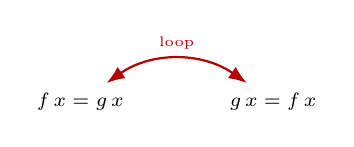
\begin{tikzpicture}[node distance=1.1cm, auto, >=Latex]
        \node (fx) {\scriptsize $f\,x = g\,x$};
        \node (gx) [right=of fx] {\scriptsize $g\,x = f\,x$};
        \draw[<->, thick, bend left=35, color=red!70!black] (fx) to node[above] {\tiny loop} (gx);
    \end{tikzpicture}
    \vspace{-0.4em}
    \end{center}

    \item Default \textbf{large library} of simp-rules:
    \begin{itemize}[leftmargin=0.8em, label=$\bullet$, itemsep=0pt]
        \item \texttt{@}, \texttt{length}, etc.
        \item Any recursive function $f$, $f.\text{simps}$ are added automatically.
    \end{itemize}
    
    \item \textbf{Manually extend} / remove simp-rules:
    \begin{center}
    \vspace{-0.2em}
    \texttt{\footnotesize apply (simp add: rule$_1$ del: rule$_2$)}
    \vspace{-0.2em}
    \end{center}
    
    \item \textbf{Note:} To remove \textit{all} facts from simpset except $f_1$:
    \begin{center}
    \vspace{-0.2em}
    \texttt{\footnotesize apply (simp only: $f_1$)}
    \vspace{-0.2em}
    \end{center}
\end{itemize}
\end{tcolorbox}

\vspace{-0.3em}

% 3. NOTES & ATTRIBUTES
\begin{tcolorbox}[title=3. Useful Notes \& Attributes]
\begin{itemize}[leftmargin=1em, itemsep=1.5pt]
    \item When proving a lemma$^a$ \texttt{lem1: "x + y = y + x"} to always use for simplification:
    \begin{center}
    \vspace{-0.2em}
    \texttt{\footnotesize lem1 [simp]: "x + y = y + x"}
    \vspace{-0.2em}
    \end{center}
    
    \item For Forward / Backward reasoning:
    \begin{center}
    \vspace{-0.2em}
    \texttt{\footnotesize lem1 [dest / intro]: ...}
    \vspace{-0.2em}
    \end{center}
    
    \item Predefined sets of simps for goal categories: E.g., \texttt{algebra\_simps}, \texttt{field\_simps}.
    
    \item \textbf{Naturals:} To translate between $\text{Suc}(\text{Suc } n)$ and $n + 2$, use:
    \begin{center}
    \vspace{-0.2em}
    \texttt{\footnotesize eval\_nat\_numerals}
    \vspace{-0.2em}
    \end{center}
\end{itemize}
\end{tcolorbox}

\columnbreak

% 2. AUTO
\begin{tcolorbox}[title=2. The \texttt{auto} Proof Method]
\begin{itemize}[leftmargin=1em, itemsep=1.5pt]
    \item \textbf{\texttt{auto} $\approx$ Simplification + Classical Reasoning}
    \begin{itemize}[leftmargin=0.8em, label=$\rightarrow$, itemsep=0pt]
        \item Simplification $\implies$ repetitive substitution
        \item Classical reasoning $\implies$ repetitive FW \& BW reasoning
    \end{itemize}
    \item Uses the \textbf{same simpset} as the simplifier.
    \item Has its own bank of \textbf{FW / BW reasoning lemmas}.
    \item \textbf{Recall:} To extend simpset for \texttt{simp}:
    \begin{center}
    \vspace{-0.2em}
    \texttt{\footnotesize apply (simp add / del / only: rule$_1$ rule$_2$ ...)}
    \vspace{-0.2em}
    \end{center}
    \item Same syntax works to modify simpset for \texttt{auto}.
    
    \item Add / remove a lemma to/from classical reasoning:
    \begin{itemize}[leftmargin=0.7em, label=--, itemsep=0pt]
        \item \texttt{\scriptsize apply (auto intro: fact$_1$)} $\rightarrow$ Adds $\text{fact}_1$ to \textbf{BW}
        \item \texttt{\scriptsize apply (auto dest: fact$_1$)} $\rightarrow$ Adds $\text{fact}_1$ to \textbf{FW}
    \end{itemize}
    
    \item \textbf{Recall:} FW reasoning is preferable for \textit{manual} proofs.
    \item \textbf{For automation:} \textbf{BW reasoning is preferable}:
    \begin{itemize}[leftmargin=0.7em, label=--, itemsep=0pt]
        \item Helps better with debugging.
        \item Usually more confident about the target conclusion.
        \item Start from conclusion \& find assumptions via BW reasoning.
    \end{itemize}
    
    \item \textbf{Note:} \texttt{auto} \textbf{applies to all open goals}, unlike \texttt{simp}, \texttt{subst}, \texttt{rule}, etc.
\end{itemize}
\end{tcolorbox}

\vspace{-0.3em}

% 4. FORCE & FASTFORCE
\begin{tcolorbox}[title=4. \texttt{force} \& \texttt{fastforce}]
\begin{itemize}[leftmargin=1em, itemsep=1.5pt]
    \item \textbf{More powerful} than \texttt{auto}.
    \item \textbf{Limitations:}
    \begin{itemize}[leftmargin=0.8em, label=--, itemsep=0pt]
        \item Cannot stop in the middle like \texttt{auto} or \texttt{simp}.
        \begin{itemize}[leftmargin=0.7em, label=$\rightarrow$, itemsep=0pt]
            \item \textbf{Not good for debugging!}
        \end{itemize}
        \item Unlike \texttt{auto}, they \textbf{only apply to the first goal}!!!
    \end{itemize}
    \item Accepts options: \texttt{simp / intro / dest ...}
\end{itemize}
\end{tcolorbox}

\end{multicols*}

\end{document}
